\let\negmedspace\undefined
\let\negthickspace\undefined
\documentclass[journal]{IEEEtran}
\usepackage[a5paper, margin=10mm, onecolumn]{geometry}
%\usepackage{lmodern} % Ensure lmodern is loaded for pdflatex
% \usepackage{tfrupee} % Include tfrupee package

\setlength{\headheight}{1cm} % Set the height of the header box
\setlength{\headsep}{0mm}     % Set the distance between the header box and the top of the text

\usepackage{gvv-book}
\usepackage{gvv}
\usepackage{cite}
\usepackage{amsmath,amssymb,amsfonts,amsthm}
\usepackage{algorithm}
\usepackage{algorithmic}
\usepackage{graphicx}
\usepackage{textcomp}
\usepackage{xcolor}
\usepackage{txfonts}
\usepackage{listings}
\usepackage{enumitem}
\usepackage{mathtools}
\usepackage{gensymb}
\usepackage{comment}
\usepackage[breaklinks=true]{hyperref}
\usepackage{tkz-euclide} 
\usepackage{listings}
% \usepackage{gvv}                                        
\def\inputGnumericTable{}                                 
\usepackage[latin1]{inputenc}                                
\usepackage{color}                                            
\usepackage{array}                                            
\usepackage{longtable}                                       
\usepackage{calc}                                             
\usepackage{multirow}                                         
\usepackage{hhline}                                           
\usepackage{ifthen}                                           
\usepackage{lscape}
% \usepackage{algpseudocode}
\begin{document}

\bibliographystyle{IEEEtran}
\vspace{3cm}

\title{NCERT 8.3.19}
\author{EE24BTECH11053 - S A Aravind Eswar}
% \maketitle
% \newpage
% \bigskip
{\let\newpage\relax\maketitle}

\renewcommand{\thefigure}{\theenumi}
\renewcommand{\thetable}{\theenumi}
\setlength{\intextsep}{10pt} % Space between text and floats

\textbf{Question:} The area bound by the y-axis, $y=\cos{x}$ and $y=\sin{x}$ when $\displaystyle 0\leq x \leq \frac{\pi}{2}$ is

\subsection{Theoretical Solution:}
    Solving $y=\cos{x}$ and $y = \sin{x}$ in the given interval, we can find that they intersect at $x = \frac{\pi}{4}$
    Thus, the area can be written as the following integral,
    \begin{align}
        A &= \int_{0}^{\pi/2} \min\cbrak{\sin{x}, \cos{x}}\, dx\\
        A &= \int_{0}^{\pi/4} \sin{x}\,dx + \int_{\pi/4}^{\pi/2} \cos{x}\,dx
    \end{align}
    Evaluvating the integral, we get,
    \begin{align}
        A = 2 - \sqrt{2}
    \end{align}

\subsection{Trapeziodal rule:}
    Let,
    \begin{align}
        \int_{a}^{b} f(x) \,dx = A
    \end{align}

    The interal can be approximated as,
    \begin{align}
        A \approx \frac{h}{2} \sum_{k=1}^{N} \brak{f(x_{k-1}) - f(x_k)}
    \end{align}

    where,
    \begin{align}
        h = \frac{b-a}{N}
    \end{align}

    Then the update equation can be written as,
    \begin{align}
        J_{n+1} = J_n + h \,\frac{f(x_{n+1}+f_n)}{2}
    \end{align}
    
    Finding the area from 0 to $\pi/4$,
    \begin{align}
        J_{n+1} &= J_n + h\, \frac{\sin{x_n} + {\sin{x_{n+1}}}}{2}\\
        x_{n+1} &= x_n + h
    \end{align}

    Giving,
    \begin{align}
        A_1 \approx 0.2926
    \end{align}

    Similarly calculating from $\pi/4$ to $\pi/2$,

    \begin{align}
        J_{n+1} &= J_n + h\, \frac{\cos{x_n} + {\cos{x_{n+1}}}}{2}\\
        x_{n+1} &= x_n + h
    \end{align}

    Giving,
    \begin{align}
        A_2 \approx 0.2926
    \end{align}

    Total Area,

    % Performing the sum interatively,
    % This can be simplified as,
    % \begin{align}
    %     A = h\brak{\frac{f(x_0) + f(x_N)}{2}+\sum_{k=1}^{N-1} f(x_k)}
    % \end{align}
    % Thus, 
    % \begin{align}
    %     \int_{0}^{\pi/2} \min\cbrak{\sin{x},\cos{x}}\,dx = h\brak{\sum_{k=1}^{N-1}\min\cbrak{\sin{x_k},\cos{x_k}}}
    % \end{align}
    
    % Taking N as 1000 and solving, we get,
    \begin{align}
        A = A_1 + A_2\\
        A \approx 0.5852
    \end{align}

    % Trapeziodal rule is given as,
    % \begin{align}
    %     y_{n+1} = y_n + \frac{h}{2}\brak{f\brak{x_n, y_n}+}
    % \end{align}

    \begin{figure}[ht]  
        \centering  
        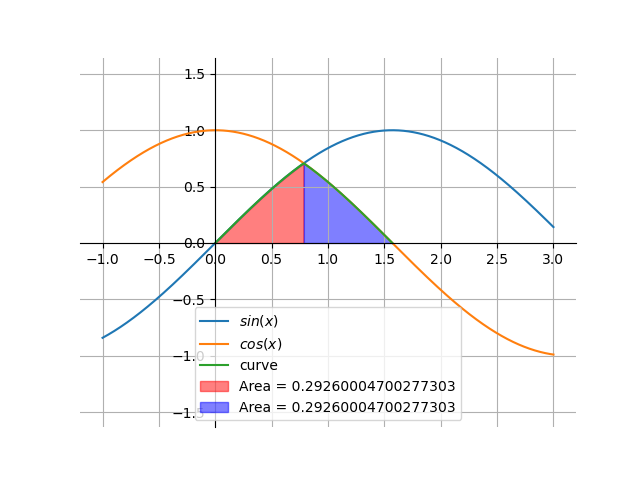
\includegraphics[width=\columnwidth]{figs/fig1.png}  
        \caption{Verification}
        % \columnwidth
    \end{figure}

\end{document}